\chapter{Analysis of Interface Roughness based on Diffuse Scattering} \label{ch_diff}
With the detailed analysis based on the combination of several complementary experimental methods and the \gls{mcmc} evaluation performed in chapter~\ref{ch_spec}, reconstructions and confidence intervals for the model parameters for all sample systems could be obtained. It was found that roughness and intermixing or interdiffusion are of high relevance to explain the diminished reflectivity observed. Most prominently, the interface morphology in the Mo/Si/C sample system from Sec.~\ref{ch_spec:sec_mo_si_c} had a large effect on the reflectivity behavior in both the polished and unpolished case. We attributed the observations to the occurrence of a crystallization process in the molybdenum layer, which affects the interface morphology. Similarly, in case of the Cr/Sc mirror system presented in Sec.~\ref{ch_spec:sec_CrSc}, intermixing or interdiffusion and roughness were attributed to cause the large gap between theoretical reflectivity predictions and actual values measured in the experiments.

So far, no distinction was made between interdiffusion or intermixing and roughness at the surface or interfaces. As discussed in detail in Sec.~\ref{ch_spec:sec_CrSc_results}, this distinction based on the employed methods is in fact not possible due to the lack of sensitivity of the experiments conducted there not even for the combination of all methods. Due to the comparatively large beam footprint on the sample in comparison to interfacial roughness on the nanoscale, any specular reflection measurement, and even the measurement of fluorescence radiation generated by a standing wave field, is only sensitive to the average of the interfacial profile and can thus not be distinguished from horizontally homogeneous intermixing. Effectively, both cases can be described with a gradual profile in the optical constants at the interfaces. Consequently, all methods applied so far rely on a horizontally homogeneous medium model, which was reconstructed. The correlation of the roughness parameter $\sigma$ and the intermixing parameter $\eta$ in Fig.~\ref{ch_spec:fig_CrSc_eta_rho_correlation} nicely demonstrate that assessment.

Within this chapter, we investigate the diffuse scattering contribution measured from all samples studied in chapter~\ref{ch_spec}. While none of the experiments conducted there could yield a distinction criterion, diffuse scattering can only be observed from rough surfaces or interfaces, while intermixing and interdiffusion do not cause any off-specular intensity contribution. The analysis of the diffuse scattering, here in particular scattering in the \gls{euv} spectral range, therefore serves as a natural tool to implement the distinction of intermixing or interdiffusion on the one hand and roughness on the other. In addition, the distribution of the scattered intensity contains information on the morphology of roughness which is of particular interest to understand the effect on the reflectivity as observed in the previous chapter. First, we continue the analysis of the Mo/B$_4$C/Si/C sample based on the reconstruction found in Sec.~\ref{ch_spec:sec_reconstruction_PTB17} and demonstrate in detail the effects observed in case of diffuse \gls{euv} scattering from multilayer systems with an analysis based on the theory introduced in Sec.~\ref{ch_theo:sec_diffuse_scattering}. In the second part, we analyze the effect of the crystallization presumed as cause for the diminished reflectivity observed for some of the samples in the two sets of Mo/Si/C systems discussed in Sec.~\ref{ch_spec:sec_mo_si_c_results}. Furthermore, the effect of the polishing process in one of the sample sets on the interface morphology is addressed. Finally, we resolve the parameter correlation of intermixing and roughness for the Cr/Sc sample and finalize the characterization made in Sec.~\ref{ch_spec:sec_CrSc_results}.


\section{Near-normal Incidence Diffuse Scattering} \label{ch_diff:sec_PTB17}
In the theoretical fundamentals on diffuse scattering in chapter~\ref{ch_theo}, we have elaborated on the characterization of the scatter intensity from a multilayer sample. The goal of the investigation of the diffuse scattering intensity is to gain information on the interface morphology in the sample. In Sec.~\ref{ch_theo:sec_elastic_scattering}, the measured scattering intensity $I_\text{s}$ is described in terms of the differential scattering cross section $\big(\frac{d \sigma}{d \Omega}\big)$, which is given explicitly for the problem of interfacial and surface roughness in multilayer samples in Eq.~\eqref{ch_theo:eqn_full_dwba_expression}. As indicated there, the full theoretical description is based on the introduction of the reciprocal space as a unique set of coordinates for the scattering problem. This space is spanned by the coordinates $q_x$, $q_y$ and $q_z$. Those are the components of the momentum transfer due to the scattering process (cf.~Sec.~\ref{ch_theo:sec_diffuse_scattering}) and are related to the experimental parameters wavelength $\lambda$, as well as the angle of incidence $\alpha_i$ and the exit angle $\alpha_f$ of the scattering experiment. Based on the theory developed in Sec.~\ref{ch_theo:sec_diffuse_scattering}, a mapping of reciprocal space along the two coordinates $q_x$ and $q_z$ is required to obtain information on the samples interface morphology.

In order to discuss the diffuse scattering experiments and enable a theoretical analysis, we shall therefore first give some definitions of measurement geometry and how it is related to the reciprocal space coordinates. So far, any scattering measurement (excluding the \gls{xrf} experiment) of chapter~\ref{ch_spec} was conducted in the specular reflection geometry, where incidence and exit angle are equal, i.e.~at $q_x = q_y \equiv 0$. Diffusely scattered radiation caused by roughness, however, is scattered to off-specular angles. The experiments conducted here are exclusively done in a co-planar geometry since the roughness in the samples under investigation are assumed to be isotropic parallel to the surface and interfaces (cf.~Sec.~\ref{ch_theo:sec_diffuse_scattering}). Thus, any scattered radiation is only measured in the scattering plane defined by the incidence wave vector and the surface normal of the multilayer sample. Two different types of measurements need to be distinguished as they relate to different paths through reciprocal space, the \emph{detector scan} geometry and the \emph{rocking scan} geometry both indicated in Fig.~\ref{ch_diff:fig_scattering_geometry}.
\begin{figure}[htb]
    \def\svgwidth{0.6\textwidth}
    \import{svg/}{Streugeometrie_diffuse.pdf_tex}
    \caption{Co-planar measurement geometries. By keeping the opening angle $\Delta\Theta$ between incident and exit beam and the detector fixed, respectively, a rocking scan can be performed by changing the sample angle $\omega$. In a detector scan the sample angle $\omega$ is kept fixed and defines the angle of incidence while the detector is moved along $\Theta$.}
    \label{ch_diff:fig_scattering_geometry}
\end{figure}
The detector scan describes a movement of the detector inside the scattering plane recording radiation scattered to the exit angle $\alpha_f$, while keeping the incidence angle $\alpha_i$ constant and is indicated by the red shaded area in Fig.~\ref{ch_diff:fig_scattering_geometry}. The rocking scan refers to a rotation of the sample around the axis perpendicular to the scattering plane while keeping the detector position fixed with respect to the incident beam (indicated by the blue shaded are in Fig.~\ref{ch_diff:fig_scattering_geometry}). The angle between detector and the incident beam is referred to as $\Delta \Theta$, while the tilt angle of the sample is $\omega$. By changing $\omega$, the incidence angle $\alpha_i$ and the exit angle $\alpha_f$ are changed accordingly. In both cases this leads to incidence and exit angles, which are no longer equal and, thus, non-vanishing values for the $q_x$ vector component. The out-of-plane angle $\theta_f$ (cf.~Fig.~\ref{ch_theo:fig_scattering_process} in Ch.~\ref{ch_theo}) remains zero in those experiments and consequently $q_y \equiv 0$.

The corresponding paths through reciprocal space are different for these two cases. They are shown schematically in Fig.~\ref{ch_diff:fig_pathsInQ} for two exemplary experimental parameter sets of incidence angle $\alpha_i$ and opening angle $\Delta \Theta$, respectively,  as well as wavelength for the two scan types.
\begin{figure}[htb]
    \def\svgwidth{0.7\textwidth}
    \import{svg/}{Qspace_paths.pdf_tex}
    \caption{Schematic positions in reciprocal space in dependence on the measurement geometry. The dashed path represents a rocking scan with the angle $\omega$. The solid line shows the movement in $q$-space when changing the detector angle $\Theta$ at a fixed angle of incidence. By tuning the wavelength at each angular position, the $q_z$-direction becomes accessible as indicated by the dotted arrows.}
    \label{ch_diff:fig_pathsInQ} 
\end{figure}
Clearly, for a mapping of the two-dimensional space spanned by $q_x$ and $q_z$ it does not suffice to perform only angular scans. In addition,wavelength scans ($\lambda$-scan) have to be performed at each angular position. By changing the wavelength and the angle in the same measurement, both degrees of freedom ($q_x$ and $q_z$) in reciprocal space become accessible.

Based on the theory in Sec.~\ref{ch_theo:sec_diffuse_scattering}, the \gls{psd} describing the statistical properties of the samples roughness contributes to the scattering intensity being only dependent on the variable $q_x$\footnote{The \gls{psd} is generally dependent on $q_\parallel = \sqrt{q_x^2+q_y^2}$, which reduces to $q_\parallel \equiv q_x$ in co-planar geometry}, i.e.~the momentum transfer within the interface planes. There, we have derived an expression for the \gls{psd}, which describes an average value across all interfaces of the multilayer. The reason for that is that due to the high quality of the multilayer system, correlation of roughness perpendicular to the stack was assumed, which we shall verify here based on the diffuse scattering experiments. Furthermore, it should be noted that individual \gls{psd}s can be described within the theoretical framework but pose an ill-defined model for the experiment conducted here. In all measurements taken here, many interfaces contribute to the diffuse scattering intensity. The experiment thus delivers a statistical average across all interfaces, which makes a distinction of individual interfaces impossible.

Based on the \gls{psd} as derived in Eq.~\eqref{ch_theo:eqn_psd} with the dependence only on $q_x$, we should expect to be able to extract its values from the measured data as cuts along the $q_x$ axis anywhere in a measured reciprocal space map. However, it was observed in grazing incidence diffuse x-ray scattering experiments, that vertical correlation of roughness causes an additional intensity modulation of the scattering in reciprocal space along the $q_z$ direction, the so-called \emph{Bragg sheets} \cite{jiang_nonspecular_1992, holy_nonspecular_1994, salditt_kinetic_1994, holy_interface_1995}.
\begin{figure*}[htb]
    \def\svgwidth{\textwidth}
    \import{svg/}{Bragg_sheets_explained.pdf_tex}
    \caption{Schematic illustration of the appearance of Bragg-sheets in the off specular scattering intensity at the $q_z$ value fulfilling the Bragg condition of the multilayer stack. The width $\delta q_z$ of the sheet is dependent on the degree of vertical correlation of roughness.}
    \label{ch_diff:fig_Bragg_sheets_explained} 
\end{figure*}
As the interfaces have periodic distances along the surface normal of the sample, roughness correlation poses an additional Bragg condition enhancing the diffuse scattering where fulfilled. The expected diffuse scattering distribution in reciprocal space is schematically depicted in Fig.~\ref{ch_diff:fig_Bragg_sheets_explained}. Since the periodicity of the interfaces is the multilayer periodicity, those Bragg sheets are expected to appear, where the first and higher order Bragg condition of the multilayer is fulfilled, i.e.~where inside the multilayer $q_z=m 2 \pi /\tilde{D}$. Here, $m$ is the integer number of the Bragg order and $\tilde{D} = \tilde{n}_i d_i + \tilde{n}_j d_j$ is the optical multilayer period thickness, where $\tilde{n}_i$ and $\tilde{n}_j$ are the real part of the index of refraction of the respective layer $i$ and $j$. Those sheets of increased intensity vary in thickness along $q_z$ depending on the strength of the correlation of roughness along the vertical direction in the sample. The higher the correlation, the thinner is the Bragg sheet in $q_z$ direction (cf.~upper and lower part of Fig.~\ref{ch_diff:fig_Bragg_sheets_explained}). In the theoretical treatment of the diffuse scattering, this vertical roughness correlation enters as a replication factor in Eq.~\eqref{ch_theo:eqn_reduced_structure_factor} and can be explicitly derived by modeling the layer growth based on the Langevin equation Eq.~\eqref{ch_theo:eqn_langevin} and is given by Eq.~\eqref{ch_theo:eqn_replication_factor}. Due to the strong enhanced intensity in those Bragg sheets, the \gls{psd} is preferably extracted as a vertical cut along $q_x$ at the $q_z$ position of the sheet \cite{salditt_kinetic_1994,siffalovic_characterization_2009}. Consequently, in the following we shall focus on the mapping of reciprocal space in the vicinity of the first Bragg resonance to observe the expected Bragg-sheet intensity distribution and analyze the interface morphology.

In the studies cited above, the reciprocal space maps of multilayer diffuse scattering have been conducted in a grazing incidence geometry using X-rays. The major disadvantage of this technique is that curved samples are not accessible in that way, since no grazing incidence measurement can be conducted if the sample is convexly curved. Here, we study the diffuse scattering using \gls{euv} radiation impinging at near-normal incidence. Thereby, this disadvantage is overcome. However, as explained above, using near-normal incidence radiation reduced the accessible $q_z$ range, which can be compensated by tuneability of the wavelength, whereas grazing incidence studies reveal the Bragg sheets in the out-of-plane direction at fixed photon energies, e.g.~\textcite{siffalovic_characterization_2009}.

\subsection{Mapping Reciprocal Space for the Mo/B$_4$C/Si/C Sample}
In this section we investigate the \gls{euv} diffuse scattering from the Mo/B$_4$C/Si/C sample discussed in Sec.~\ref{ch_spec:sec_PTB17} as an example for the analysis of near-normal scatter intensity from multilayer samples. We have conducted diffuse scattering measurements in three different geometries at the \gls{sx700} beamline at \gls{bessy}. From the experimental data, the respective reciprocal space coordinates were calculated and the corresponding maps and the experimental details are given in Fig.~\ref{ch_diff:fig_PTB17_detector_and_rocking_maps}.
\begin{figure*}[htbp]
        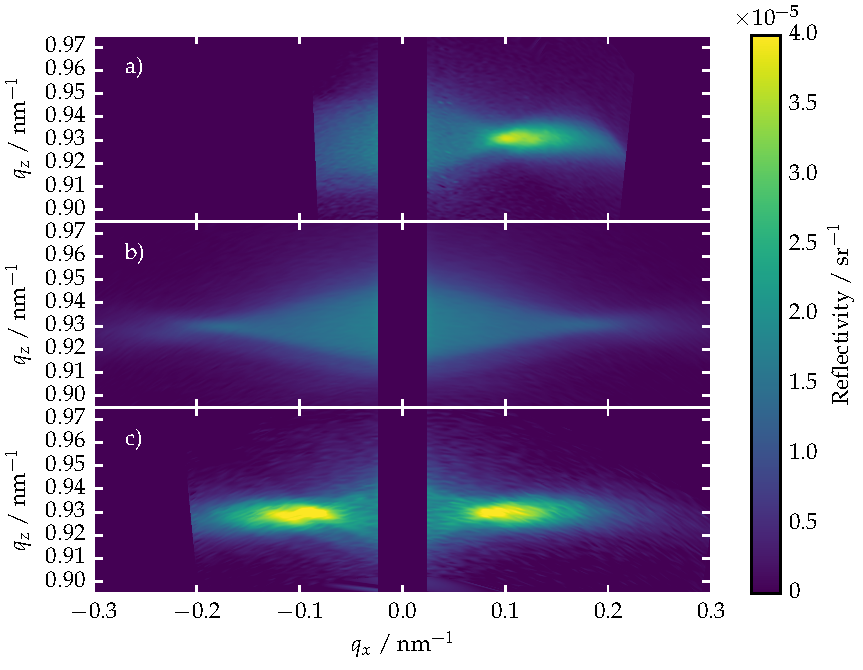
\includegraphics[width=
        \textwidth]{img/PTB17_diffuse_scattering_multiple_geometries} \caption{Measured intensity map of a detector scan of the Mo/B$_4$C/Si/C multilayer mirror at an angle of incidence $\alpha_i = 6.75^\circ$ (a) and measured intensity maps of the identical sample obtained through rocking scans at an opening angle between detector and incident beam of $\Delta \Theta = 13.5^\circ$ (b) and $\Delta \Theta = 30^\circ$ (c). The area close to the specular axis was excluded from this dataset due to its strong intensity compared to the diffuse scattering shown here. The access to the negative $q_x$-axis in (a) is limited due clipping of the incoming beam with the detector.
        A GaAsP photo diode with an active area of $\mm{4.5} \times \mm{4.5}$ at a distance to the sample of $\mm{250}$ was used as a detector for the diffusely scattered radiation. The reciprocal space maps were recorded for the two rocking scan geometries (b,c) with at an opening angle of $\Delta \Theta = 13.5^\circ$  and of $\Delta \Theta = 30^\circ$ (corresponding to an angle of incidence of $\alpha_i = 6.75^\circ$ and $\alpha_i = 15.0^\circ$, respectively, in specular geometry), respectively, and for the detector scan geometry (a) with the angle of incidence fixed at $\alpha_i = 6.75^\circ$. The first Bragg peak for this multilayer sample, due to its design, is in the wavelength range between \nm{12.4} and \nm{14.0}. At each angular position of the aforementioned angular scan geometries, a wavelength scan was conducted in this range using a step size of $\Delta \lambda = \nm{0.01}$. The angular ranges for the rocking scan with opening angle $\Delta \Theta = \SI{13.5}{\degree}$ correspond to angles of incidence from $\alpha_i = \SI{-18.0}{\degree}$ to $\alpha_i = \SI{31.5}{\degree}$ in steps of $\Delta\alpha_i = \SI{0.5}{\degree}$. In terms of the rocking angle $\omega$ this range corresponds to values from $\omega = \SI{-24.75}{\degree}$ to $\omega = \SI{24.75}{\degree}$, where $\omega = \SI{0.0}{\degree}$ corresponds to the specular reflection geometry ($\alpha_i = \alpha_f$). For the second rocking scan geometry with $\Delta \Theta = \SI{30.0}{\degree}$, the angle of incidence was varied from $\alpha_i = \SI{-3.0}{\degree}$ to $\alpha_i = \SI{27.5}{\degree}$ (corresponding to $\omega = \SI{-18.0}{\degree}$ to $\omega = \SI{12.5}{\degree}$) in steps of $\SI{0.5}{\degree}$. Finally, the detector scan was performed at an angle of incidence of $\alpha_i = \SI{6.75}{\degree}$ moving the detector from $\alpha_f = \SI{-3.75}{\degree}$ to $\alpha_f = \SI{46.75}{\degree}$ (corresponding to detector angles from $\Delta \Theta = \SI{3.0}{\degree}$ to $\Delta \Theta = \SI{40.0}{\degree}$) also in steps of $\SI{0.5}{\degree}$.} \label{ch_diff:fig_PTB17_detector_and_rocking_maps}
\end{figure*}

The reciprocal space maps in Fig.~\ref{ch_diff:fig_PTB17_detector_and_rocking_maps} for the rocking scan (b) at an opening angle of $\Delta \Theta = 13.5^\circ$ and the rocking scan (c) at an opening angle of $\Delta \Theta = 30^\circ$ and for the detector scan with the angle of incidence $\alpha_i = 6.75^\circ$ clearly show different symmetries rather than the expected Bragg sheet. We observe a strong enhancement in the off-specular scattering around $q_x\approx \pm 0.1$ nm$^{-1}$ (cf.~(a) and (c)), which is not replicated on the negative $q_x$-axis in case of (a). The rocking scans (b) and (c) are symmetric with respect to the specular axis at $q_x=0$, however, no enhanced scattering appears in (b). The latter map shows a triangular-shaped intensity distribution for both the positive and 
negative $q_x$ range. A minimum in the width with respect to the $q_z$ direction can be observed here around $q_x \approx \pm 0.2$ nm$^{-1}$. The triangular shape also appears for the 
positive $q_x$ range 
of the detector scan in (a), where the minimum in width coincides with the intensity maximum. These observations are in clear contrast to the expectation of an appearance of identical Bragg sheets, independent of the measurement geometry. Clearly, the measurement of diffuse scattering at \gls{euv} wavelengths and near-normal incidence differs from the observations made for grazing incidence experiments using X-rays (cf.~\textcite{salditt_kinetic_1994} or \textcite{jiang_nonspecular_1992}).

The measurement geometry dependence of the reciprocal space maps indicates that the intensity distributions cannot be the result of multilayer roughness properties alone, i.e.~the \gls{psd}. Scattering intensities caused by roughness occur at identical positions in reciprocal space for any measurement geometry. In fact, the additional modulations of the scatter intensity are caused by the direction from which the radiation impinges on the multilayer structure itself, rather than the roughness properties. Starting from the theoretical description, the contributions observed here are therefore clearly a direct result of the field amplitudes at the interfaces as described in the theory chapter~\ref{ch_theo:sec_diffuse_scattering} entering the full expression for the differential scattering cross section in Eq.~\eqref{ch_theo:eqn_full_dwba_expression}. To better understand the effects involved here, we shall analyze the intensity curves for all three measurement geometries based on a horizontal cut along $q_x$ at the position of $q_z=\SI{0.93}{\nano\meter^{-1}}$, which corresponds to the momentum transfer at the multilayer resonance and thus the maximum of the Bragg sheet and contain the \gls{psd} analogous to \textcite{siffalovic_characterization_2009}. The intensity curves are shown in direct comparison in Fig.~\ref{ch_diff:fig_PTB17_qx_cuts_different_geometries}.
\begin{figure}[htbp]
	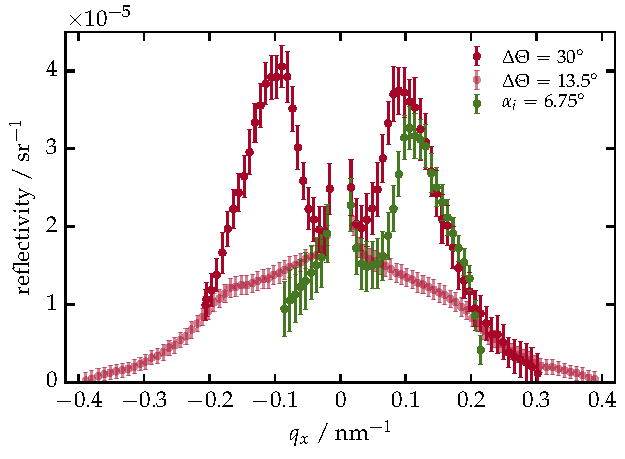
\includegraphics{img/PTB17_diffuse_BraggSheet_DetectorAndRocking} \caption{Averaged diffuse scattering intensity along $q_x$ in the interval  $q_z=(0.930 \pm 0.003$) nm$^{-1}$ corresponding to the resonance of the multilayer. The data shown are two rocking scan and one detector scan geometries (see text for details).} \label{ch_diff:fig_PTB17_qx_cuts_different_geometries}
\end{figure}
The strong off-specular enhancement of scattering intensity is clearly visible here for the detector scan geometry and the rocking scan with opening angle of $\Delta\Theta = \SI{30.0}{\degree}$. In case of the second rocking scan with $\Delta\Theta = \SI{13.5}{\degree}$, only a small shoulder can be observed at $q_x \approx \pm \SI{0.2}{\nano\meter^{-1}}$.

\subsection{Kiessig-like Peaks and Resonant Effects}
To explain the observed off-specular intensity distribution for the multilayer sample investigated here, additional effects exceeding the description of Bragg sheets need to be taken into account. So far, the description of diffuse scattering and enhancement due to correlated roughness was under the assumption of kinematic scattering, i.e.~a single diffuse scattering event. However, multiple reflections at the interfaces may not be ignored. To clarify that, we shall consider two additional processes, which may happen before and after a diffuse scattering event at the interface. Fig.~\ref{ch_diff:fig_kiessig_like_peaks_scheme} illustrates two situations, where the impinging or exiting (diffusely scattered) radiation is in resonance with the multilayers Bragg condition, i.e.~strongly enhanced in intensity.
\begin{figure*}[htb]
    %\def\svgwidth{\textwidth}
    \import{svg/}{Bragg_sheet_sheme.pdf_tex}
    \caption[Illustration of dynamic scattering processes]{Illustration of dynamic scattering processes. In (a), the impinging radiation is resonantly reflected from the multilayer structure by fulfilling the Bragg condition. In (b), certain parts of the diffusely scattered radiation from the interface roughness again fulfills the Bragg condition and is enhanced in intensity.}
    \label{ch_diff:fig_kiessig_like_peaks_scheme}
\end{figure*}
In the first case (a), the impinging radiation fulfills the Bragg condition with respect to angle of incidence and is consequently resonantly reflected from the multilayer mirror. Through this, any diffusely scattered radiation measured at any exit angle would be significantly stronger compared to the situation, where the incidence angle or wavelength do not fulfill the Bragg condition, despite the fact that the roughness itself did not change. In the second case (b), depending on the wavelength some of the diffusely scattered radiation fulfills the Bragg condition of the multilayer and is again reflected resonantly from it causing a major intensity increase.

Those effects are the result of multiple (dynamic) reflections inside the multilayer system. They were observed as resonantly enhanced streaks, so-called \emph{Bragg-like lines}, and intense \emph{Bragg-like peaks}, where both the conditions illustrated in Fig.~\ref{ch_diff:fig_kiessig_like_peaks_scheme} are fulfilled. Often observed in diffuse scattering maps from multilayer samples recorded in grazing incidence geometry with X-rays  \cite{holy_nonspecular_1994}. The theoretical principle leading to these off-specular enhancements is also known as the process of \emph{Umweganregung} \cite{baumbach_influence_1994, baumbach_grazing-incidence_1995}. As the fulfillment of the Bragg condition is only dependent on two of the three experimental parameters, i.e.~either the incidence angle $\alpha_i$ or the exit angle $\alpha_f$ in both cases together with the wavelength, the position of those enhancements is different in the reciprocal space map depending on the measurement geometry. In literature \cite{holy_nonspecular_1994, mikulik_x-ray_1997, baumbach_influence_1994, baumbach_grazing-incidence_1995}, such enhancements were so far only observed from the main Bragg resonance of the multilayer. In our case no higher order Bragg resonances can be observed, as they would appear as Bragg-like peaks in the off-specular scattering far away from the accessible $q$-space range of our experiment. However, the two Bragg-like lines corresponding to the first order Bragg peak cross at the position of the specular reflex and otherwise amount to broad bands in the diffuse map as we shall elaborate in the following.

\begin{figure}[htbp]
        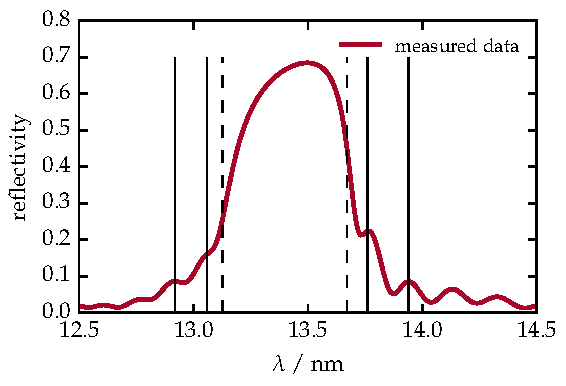
\includegraphics{img/kiessig_like_peaks_reflectivity_curve} \caption{Measured reflectivity curve of the Mo/B$_4$C/Si/C multilayer mirror at an angle of incidence $\alpha_i = 6.75^\circ$. The solid black lines mark the positions of the first two Kiessig-fringes at each side of the main maximum. The dashed lines indicate the \gls{fwhm} position of the main Bragg peak.}
        \label{ch_diff:fig_ptb17_reflectance_AOI_675} 
\end{figure}
Apart from the main Bragg peak, additional resonances are observed in the \gls{euv} reflectivity curve as shown in Fig.~\ref{ch_diff:fig_ptb17_reflectance_AOI_675}. Those side peaks, known as Kiessig fringes \cite{kiessig_interferenz_1931} as previously discussed in Sec.~\ref{ch_spec:sec_PTB17}, correspond to the interference of radiation reflected from the top surface and the substrate interface. The dynamic enhancement expected for those side fringes is very well within the measured reciprocal space ranges for the experimental geometries and wavelengths. In Fig.~\ref{ch_diff:fig_kiessig_like_peaks_diffuse_map} the positions where those enhancements are expected in the maps shown in \ref{ch_diff:fig_PTB17_detector_and_rocking_maps} are indicated as white solid lines for the first two fringes on either side of the reflectivity curve maximum. In addition, the \gls{fwhm} of the main Bragg maximum was marked with dashed lines.
\begin{figure*}[htbp]
        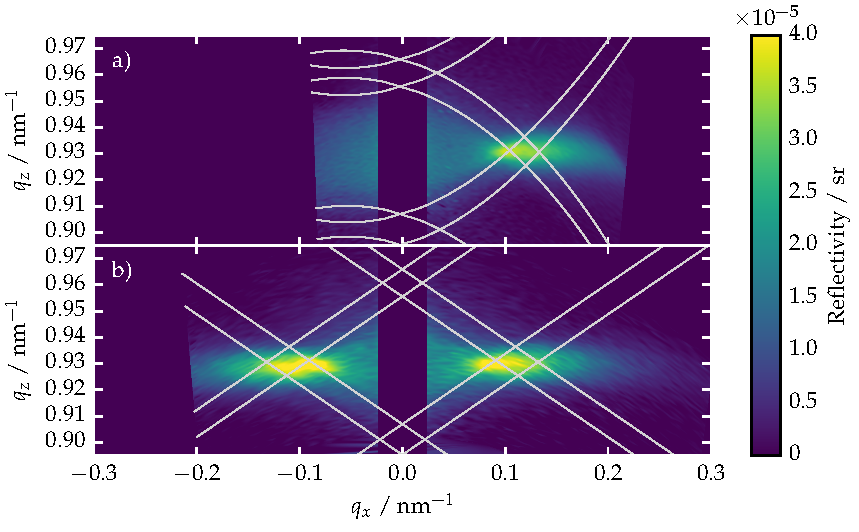
\includegraphics[width=\textwidth]{img/kiessig_like_peaks_diffuse_map} \caption{Measured intensity maps of Fig.~\ref{ch_diff:fig_PTB17_detector_and_rocking_maps} with the calculated positions of the Kiessig-like lines (solid lines) for the Kiessig fringes marked in Fig.~\ref{ch_diff:fig_ptb17_reflectance_AOI_675} and the Bragg-like lines (bands between the dashed lines). The positions, where the solid lines cross show the Kiessig-like peaks positions. The area contained within the dashed lines in the center of each plot correspond to the Bragg-like peak of the first Bragg order of the multilayer and explain the triangular or diamond shaped area of increased intensity (see main text).} \label{ch_diff:fig_kiessig_like_peaks_diffuse_map} 
\end{figure*}
Clearly, the off-specular enhancement observed fits to the theoretically predicted appearance of Bragg-like peaks, i.e.~at the crossing points of the lines, which we shall call \emph{Kiessig-like peaks}, due to their origin. The strong enhancement, however, is only observed where there is also a Bragg sheet due to correlated roughness. The aforementioned broad bands corresponding to the Bragg-like lines of the main Bragg resonance appear in between the dashed lines. Indeed, most prominently visible in Fig.~\ref{ch_diff:fig_kiessig_like_peaks_diffuse_map}b, the triangular shaped intensity distribution in the center of the map is in fact the results of resonant enhancement due to the first order Bragg-like peak, which extents across a large area of the map in this case.
The diffuse scattering distribution in the reciprocal space maps is thus a combination of dynamic effects (the first-order Bragg-like peak and the Kiessig-like peaks) and kinematic effects~(Bragg sheets).

The processes described here are contained in the theoretical description given in Eq.~\eqref{ch_theo:eqn_full_explicit_dwba_with_approximations} in Sec.~\ref{ch_theo:sec_diffuse_scattering}\footnote{They correspond to the contributions of the \gls{dwba} differential cross section through the processes shown in Fig.~\ref{ch_theo:fig_dwba_scheme}, labeled $R T^*$ and $T R^*$ (Kiessig-like lines, Bragg-like lines) and $R R^*$ (Kiessig-like peaks, Bragg-like peaks)}. In order to assess the contribution of dynamic multiple reflections within the stack, we compared the semi-kinematic approximation in Eq.~\eqref{ch_theo:eqn_semi_kinematic_dwba_expression} with the dynamic calculations in Eq.~\eqref{ch_theo:eqn_full_explicit_dwba_with_approximations}. In the semi-kinematic case, all multiple reflection effects are ignored in the differential cross section. The result is the intensity distribution as expected from the kinematic case, however including the accurate transmitted field amplitudes at each interface instead of only a plane wave field amplitude as in the simple Born approximation. For this comparison, we simulated the rocking scan at an opening angle of $\Delta \Theta = 30^\circ$. The roughness properties for these simulations were determined following the procedure described below in Sec.~\ref{ch_diff:sec_determination_of_the_psd} to match the samples properties\footnote{In Sec.~\ref{ch_spec:sec_reconstruction_PTB17}, a reconstruction based on the measurement of \gls{euv} reflectivity curves was found and the values listed in table~\ref{ch_spec:tbl_mo_b4c_si_c_multilayer_mcmc_results} serve as the model parameters for the analysis conducted here.}.

To evaluate the contribution of multiple reflections due to the subsidiary maxima, Fig.~\ref{ch_diff:fig_kiessig_like_peak_along_qx}b shows the intensity distribution along $q_x$ at $q_z=0.93$ nm$^{-1}$ again in comparison to the \gls{euv} reflectivity curve in Fig.~\ref{ch_diff:fig_kiessig_like_peak_along_qx}a.
\begin{figure*}[htbp]
        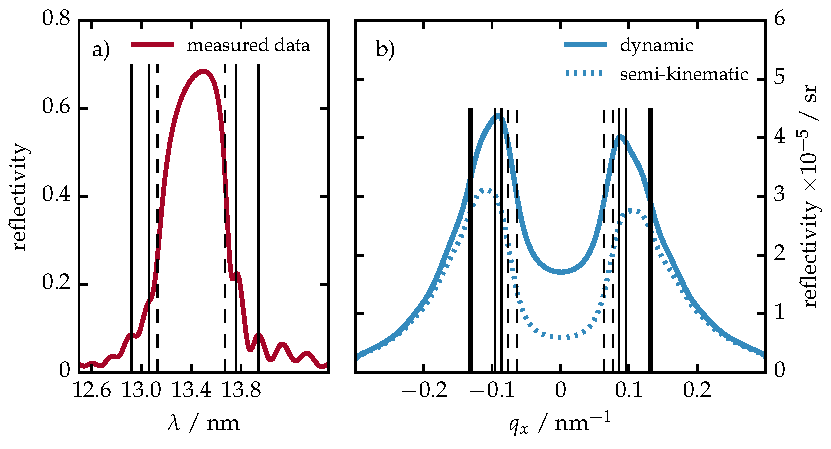
\includegraphics[width=\textwidth]{img/qx_kinematic_vs_dynamic}
        \caption{a) \gls{euv} reflectivity curve with the positions of the \gls{fwhm} of the Bragg peak (dashed black lines) and the positions of the first two Kiessig fringes on each side of the main maximum (solid black lines) similar to Fig.~\ref{ch_diff:fig_ptb17_reflectance_AOI_675}. b) Calculated scattering intensity distribution at $q_z=0.93$ nm$^{-1}$. The solid blue line shows the result of the dynamic calculation for a rocking scan with an opening angle of $\Delta\Theta=30^\circ$. The dashed blue line represents the calculation applying the semi-kinematic approximation, ignoring any multiple reflections within the multilayer. The dashed vertical lines are the position of the main Bragg peaks \gls{fwhm}, while the solid vertical lines show the position of dynamic contributions of the Kiessig fringes close to the main maximum. Each Kiessig fringe marked in the inset appears for the corresponding positive and negative $q_x$ value. The strong intensity at $q_x\approx0.1$ nm$^{-1}$ results from the overlap of the dynamic maxima of two different Kiessig fringes (see text).} \label{ch_diff:fig_kiessig_like_peak_along_qx} 
\end{figure*}
The solid blue line corresponds to the dynamic theory, while the dotted blue line is the result of the semi-kinematic calculation. The dashed vertical lines indicate the limits of the main Bragg peaks \gls{fwhm}. The vertical black lines show the position of the Kiessig-like lines intersecting the cut position. Each of the marked fringes in Fig.~\ref{ch_diff:fig_kiessig_like_peak_along_qx}a appears on the negative and positive $q_x$-axis in Fig.~\ref{ch_diff:fig_kiessig_like_peak_along_qx}b. This is caused by the incidence and exit angle, respectively, being at the resonance angle of the various Kiessig maxima in the reflectivity curve as illustrated in Fig.~\ref{ch_diff:fig_kiessig_like_peaks_scheme}. A strong increase with respect to the semi-kinematic approximation is observed. The position of the dynamic contribution from the first 
Kiessig fringes on either side of the main resonance exhibits a pronounced maximum in the diffuse scattering. These fringes contribute most due to their high overall relative 
intensity compared with the fringes further away from the reflectivity maximum. In addition, the position in reciprocal space coincides with the first two Kiessig fringes marked on either side of the main maximum. The contribution by the main Bragg resonance, i.e.~the Bragg-like peak amounts to approximately 100\% at $q_x=0$. The comparison to the semi-kinematic case reveals another reason for the strong intensity of the Kiessig-like peaks compared to the Bragg-like peak. In between the dashed lines on the positive and negative $q_x$ axis in Fig.~\ref{ch_diff:fig_kiessig_like_peak_along_qx}b, a significant decrease of kinematically scattered radiation is observed. The reason for that is a strongly diminished penetration depth of the radiation into the multilayer at the Bragg resonance, which causes less rough interfaces to contribute to the diffuse scattering. This directly counteracts the resonant enhancement due to the Bragg-like peak and leads to an overall lower scattering contribution at these positions in reciprocal space.

A quantitative comparison of the dynamic contribution to the total scattering intensity in our measurements is shown in Fig.~\ref{fig:Comparison_full_semi} as a line cut along the $q_z$ at $q_x=0.05$ nm$^{-1}$, perpendicular to the simulations shown in Fig.~\ref{ch_diff:fig_kiessig_like_peak_along_qx}.
\begin{figure}[htbp]
        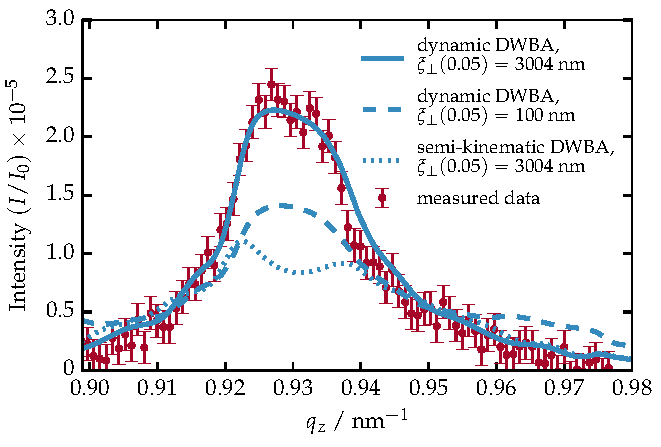
\includegraphics{img/PTB17_diffuse_qz_kinematic_vs_dynamic_100nm} \caption{Scattering intensity along $q_z$ for $q_x=0.05$ nm$^{-1}$ for the dynamic and semi-kinematic calculations for a rocking scan at $\Delta\Theta=30^\circ$ in comparison to the measured data.} \label{fig:Comparison_full_semi} 
\end{figure}
The dynamic calculation yields excellent agreement with the measured data with the \gls{psd} and correlation parameters obtained following the procedure explained in Sec.~\ref{ch_diff:sec_determination_of_the_psd}. The results show distinct differences with an increase up to 100\% of the scattered intensity close to the multilayer resonance at $q_z=0.93$ nm$^{-1}$ compared to the semi-kinematic calculation. Hence the dominance of the dynamic contributions in the vicinity of the Bragg resonance is also observed here. In addition to comparing the dynamic and semi-kinematic calculations, a dynamic calculation assuming a reduced vertical correlation of roughness was added as dashed blue curve. As discussed in the beginning of Sec.~\ref{ch_diff:sec_PTB17}, the Bragg sheet width is strongly dependent on the amount of correlated interfaces. Clearly, a broadening and reduction of scatter intensity is seen for this case here. This shows, that the Bragg sheet is in fact still visible but obscured by the dominant structure in the diffuse scattering caused by the dynamic effects explained above.

\subsection{Reconstruction of the PSD and the Multilayer Enhancement Factor}
\label{ch_diff:sec_determination_of_the_psd}
The large impact of resonant effects on the off-specular scattering intensity measured in the three geometries shown above prove, that multiple reflections have to be taken into account to extract the contribution of the interface morphology and determine a \gls{psd}. In the theoretical treatment of the diffuse scattering, we have derived an expression for the differential cross section based on the \gls{dwba}. It separates the dynamic enhancements and penetration depth considerations from the power spectral density contribution. The corresponding equation (cf.~Eq.~\eqref{ch_theo:eqn_full_explicit_dwba_with_approximations}), is given by
    \begin{align}
        {\underset{\text{DWBA}}{\Big(\frac{d \sigma}{d \Omega}\Big)}} = &\textcolor{fit_color}{\Bigg[\frac{A \pi^2}{\lambda^4}\sum \limits_{j=1}^{N}\sum \limits_{i=1}^{N} (n_j^2 - n_{j+1}^2)^* (n_i^2 - n_{i+1}^2)\Big( (T^{(1)}_j + R^{(1)}_j)^* (T^{(2)}_j + R^{(2)}_j)^*} \nonumber \\ &\textcolor{fit_color}{\qquad\times(T^{(1)}_i + R^{(1)}_i) (T^{(2)}_i + R^{(2)}_i) \Big) \exp\Big(-i q_x \tan \beta (z_i-z_j)\Big) c_\perp^{i j}\Bigg]}\,\, \textcolor{data_color}{C(q_x)} \text{.} \label{ch_diff:eqn_full_explicit_dwba_with_approximations}
    \end{align}
The equation is colored to indicate the two parts of interest. The blue colored factor contained in rectangular brackets is the dynamic and kinematic part due to the scattering properties from a multilayer and only dependent on the multilayer layout, we therefore refer to it as \emph{multilayer enhancement factor}. The red colored term $\textcolor{data_color}{C(q_x)}$, is the average power spectral density and describes the average interface morphology.

To illustrate the impact due to the presence of the multilayer and the geometry dependence, the result of calculations of the multilayer enhancement factor alone, based on the layer model of our multilayer sample is shown in Fig.~\ref{ch_diff:fig_PTB17_multilayer_enhancement_factor} for the detector scan and the two rocking scan configurations. The multilayer enhancement factor was normalized with respect to $q_x=0$, i.e. the calculated diffuse scattering contribution on the specular axis.
\begin{figure}[htbp]
	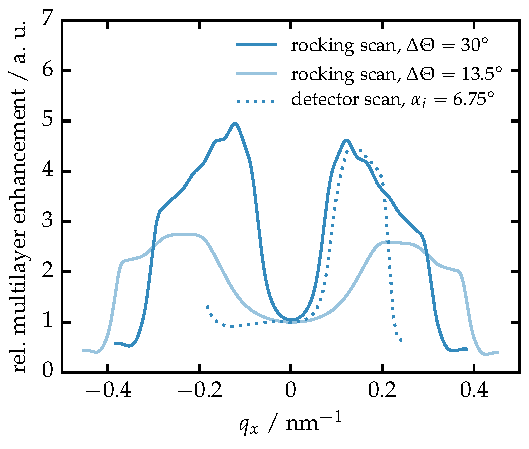
\includegraphics{img/PTB17_multilayer_enhancement_factor} \caption{Enhancement factor due to the specific properties of multilayer reflectivity for three different measurement geometries. The simulations shown here were normalized with respect to the diffuse contribution to the specular reflectivity at $q_x=0$.} \label{ch_diff:fig_PTB17_multilayer_enhancement_factor} 
\end{figure}

The results show that the diffuse scattering from these multilayer mirrors systems at near-normal incidence exhibits strong enhancement due to the intrinsically limited bandpass of reflectivity. If both the incidence and exit angle is out of the Bragg resonance, the higher penetration depth of the multilayer causes an increase in the number of interfaces contributing to the diffuse scattering intensity. Thus higher total scattering is observed. The Kiessig fringes and the main Bragg peak cause modulations in the enhancement factor increased by the purely dynamic processes described in the previous section. Based on the results, the cuts along $q_x$ shown in Fig.~\ref{ch_diff:fig_PTB17_qx_cuts_different_geometries} through the three measured maps from this sample could be normalized to extract the \gls{psd} of the sample. The result is shown in Fig.~\ref{ch_diff:PTB17_PSD_for_all_geometries} for the positive $q_x$ range.
\begin{figure}[htbp]
	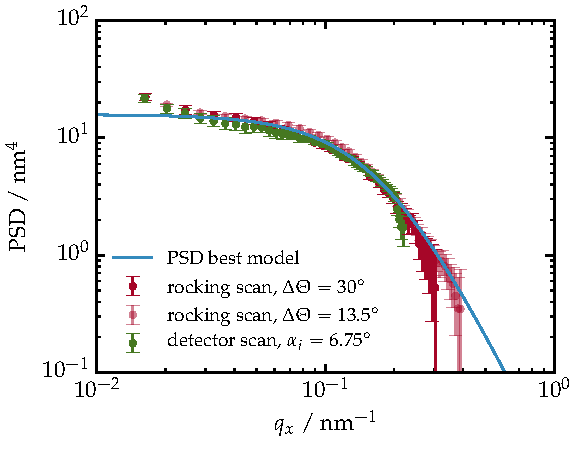
\includegraphics{img/PTB17_PSD_for_all_geometries} \caption{Diffuse scattering intensity corrected for the multilayer enhancement factor. The blue solid line corresponds to a power spectral density with $\xi_\parallel=5.6$ nm, $H=1.0$, $\sigma=0.2$ nm and a vertical correlation length of $\xi_\perp(q_x)=7.5/q_x^2$ nm$^{-1}$.} \label{ch_diff:PTB17_PSD_for_all_geometries} 
\end{figure}
Clearly, this result shows a consistent determination for the \gls{psd}, with the individual cuts being in agreement withing the measurement uncertainty. Based on the calculation of the multilayer enhancement factor, experimental curves for the \gls{psd} can be extracted as shown in Fig.~\ref{ch_diff:PTB17_PSD_for_all_geometries} without applying a specific model for the interface morphology. However, the measurements conducted here only deliver data in a limited range in the reciprocal space, depending on the selected geometry and wavelengths. To characterize the interface morphology, it is therefore necessary to model the measured data and deduct parameters that relate to the roughness properties. To obtain the \gls{psd} best model reconstruction, the \gls{pso} method was employed similarly to the reconstructions shown in the previous chapter. The details of this analysis will be given in the following paragraph.

\subsubsection{Reconstruction of the Power Spectral Density}
Within the framework of the \gls{dwba}, considering the dynamic effects, the full expression for the differential cross section of the diffuse scatter is given in Eq.~\eqref{ch_diff:eqn_full_explicit_dwba_with_approximations}. As discussed above, the power spectral density only becomes accessible through the diffuse scattering measurements, if the structural properties of the multilayer are known. Those were determined for all samples in this thesis with the methods described in chapter~\ref{ch_spec}. Based on those results, the differential cross section allows to calculate the scattering intensity maps, which were measured here and therefore enable the reconstruction of the \gls{psd}.

It is the goal of this analysis to deduct key properties of the interface roughness, such as vertical and lateral correlations and the \gls{rms} roughness value $\sigma_r$. The latter is directly related to the N\'{e}vot-Croce parameter $\sigma$, while there intermixing at the interfaces is also contained as it can not be distinguished from the roughness. Based on the analysis of the \gls{psd}, this distinction can be made. To reconstruct the \gls{psd}, a suitable model has to be introduced for the interface morphology. Here, we apply a fractal interface model, which was found to adequately describe the roughness in case of sputter deposited multilayer systems \cite{de_boer_x-ray_1995, de_boer_x-ray_1996, sinha_x-ray_1988}. It should be noted, that the \gls{psd} for a two dimensional surface should be two-dimensional itself and consider possibly different roughness properties in $x$ ($q_x$) and $y$ ($q_y$) direction. The samples we are investigating here, however, are fabricated using magnetron sputtering and on rotating sample holders as shown in Sec.~\ref{ch_exp:sec_magnetron_sputtering}. This is important to achieve a homogeneous deposition. We therefore conclude, that roughness on the surfaces and interfaces does not have any predominant direction and may be assumed to be isotropic, i.e.~only dependent on the absolute value of the lateral momentum transfer vector $q_\parallel = \sqrt{q_x^2+q_y^2}$. The \gls{psd} can then be expressed in the closed analytical one-dimensional form as shown in Eq.~\eqref{ch_theo:eqn_psd}. The three parameters describing the fractal nature of the roughness are the lateral correlation length $\xi_\parallel$, the \gls{rms} roughness $\sigma_r$ and the Hurst factor $H$. The vertical correlation of the roughness parameter $\xi_\perp$ and the off-axis roughness correlation angle $\beta$, however, are not included in the \gls{psd} as they are part of the multilayer enhancement factor. In order to fully characterize the system, we therefore analyze the full data set comprising all data points measured for the reciprocal space maps. As explained above, the maps were measured by performing wavelength scans at each angular position of the rocking or detector scans. The result are intensity curves $I_{(\alpha_i, \alpha_f)}(\lambda)$, for each set of angular positions in dependence on the wavelength. The minimization functional $\tilde{\chi}^2$ for each of the three experiments (three diffuse scattering maps), is thus given by
\begin{align}
 \tilde{\chi}^2 = \frac{1}{M-P} \sum\limits_{(\alpha_i, \alpha_f)} \sum\limits_{m} \frac{\big(I_m^\text{model}(\alpha_i, \alpha_f, \lambda)
- I_m^\text{meas}(\alpha_i, \alpha_f, \lambda)\big)^2}{\tilde{\sigma}_m^2} \text{,}
\end{align}
where $M$ is the total number of measurement points, $P$ is the number of optimization parameters and $(\alpha_i, \alpha_f)$ indicates a specific position in the angular detector or rocking scans. The reconstruction was achieved by applying the \gls{pso} technique on the combined set of measurements from all three experiments, i.e.~minimizing the functional $\chi^2 = \tilde{\chi}^2_\text{a} + \tilde{\chi}^2_\text{b} + \tilde{\chi}^2_\text{c}$. The letter indices a, b and c refer to the reciprocal space maps shown in Fig.~\ref{ch_diff:fig_PTB17_detector_and_rocking_maps}. The optimization model parameters are listed in table~\ref{ch_diff:tbl_PTB17_diffuse_optimization_limits_and_results} together with the converged results found.
\begin{table*}
\centering
\caption{Parameters of the DWBA analysis. The lower bound (LB) and upper bound (UB) specify the \gls{pso} parameter space limits.}
\label{ch_diff:tbl_PTB17_diffuse_optimization_limits_and_results}
\begin{tabularx}{\textwidth}{@{}lXrrr@{}}
\toprule
Parameter & Definition & LB & UB & PSO result\\ \midrule
$\sigma_r$ / nm & root mean square roughness & $0.0$& $1.0$ & $0.201$\\ 
$\xi_\parallel$ / nm & lateral correlation length & $0.0$& $20.0$ & $5.579$\\ 
$\xi_\perp$ / nm$^{-1}$ &vertical correlation parameter yielding vertical correlation length trough $\tilde{\xi}_\perp(q_\parallel) = \xi_\perp/q_\parallel^2$ &$0.0$ & $20.0$ & $7.512$\\
$\beta$ / $^\circ$&angle for off-axis vertical roughness correlation& $-10.0$ & $10.0$ & $-0.152$\\ 
 \bottomrule
\end{tabularx}
\end{table*}
In Fig.~\ref{ch_diff:fig_PTB17_diffuse_comparisonWithTheory}, the detector scan geometry and the rocking scan geometry measured reciprocal space maps are shown in direct comparison with the theoretically calculated maps based on the best model results. 
\begin{figure*}[htbp]
        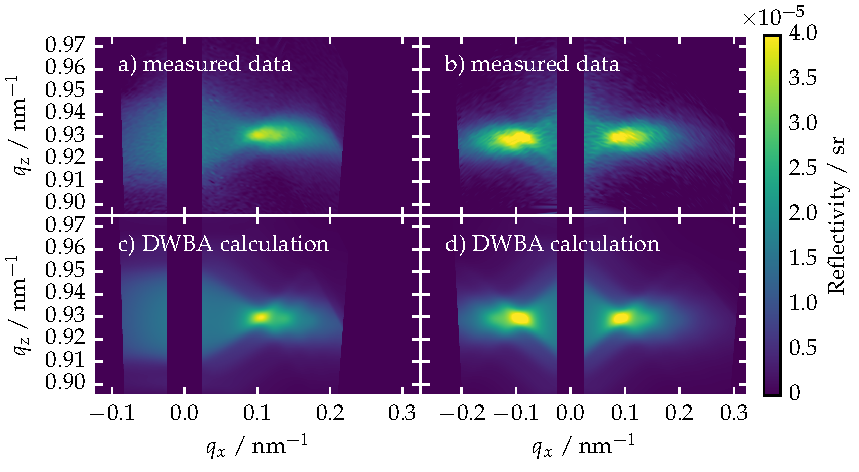
\includegraphics[width=
        \textwidth]{img/PTB17_diffuse_simulation_vs_measurement} \caption{Measured  reciprocal space maps for the detector scan geometry (a) and the rocking scan at an opening angle of $\Delta\Theta=30^\circ$ (b). The corresponding calculated maps based on the \gls{pso} results are shown in direct comparison in (c) and (d) for the respective scan geometries.} \label{ch_diff:fig_PTB17_diffuse_comparisonWithTheory} 
\end{figure*}
The direct comparison shows a good agreement of the calculated reciprocal space maps with the measured data. The results reveal a strong correlation of the roughness throughout the multilayer stack. Indeed, the correlation length extends across the whole multilayer stack up to spacial frequencies of $q_\parallel \approx \SI{0.13}{\nano\meter^{-1}}$. Beyond that frequency the correlation length reduces to values lower than the total stack thickness according to the relation $\tilde{\xi}_\perp(q_\parallel) = \xi_\perp / q_\parallel^2$. The average \gls{psd} parameters obtained show a \gls{rms} roughness of $\sigma_r=\nm{0.201}$, which is in agreement with the value $\sigma = \nm{0.214} (-\nm{0.143} / +\nm{0.201})$ obtained in the \gls{mcmc} analysis conducted in Sec.~\ref{ch_spec:sec_reconstruction_PTB17} for the N\'{e}vot-Croce parameter. In thus may be concluded that roughness is the dominant disturbance relevant for diminished reflectivity for that sample and the interdiffusion barriers provide effective means to hinder intermixing.

In conclusion, the analysis of diffuse scatter presented here provides a powerful method for the reconstruction of the average \gls{psd} of the interfaces inside the multilayer. In comparison to techniques such as \gls{afm}, which solely measure at the top surface, it can deliver data on the interface properties inside the multilayer. In addition it provides information on a large area of the surface and the interfaces. The near-normal incidence angles used in the measurement allow to study potentially strongly curved multilayer mirrors, which are often implemented in optical setups, and thus provides an advantage to established grazing-incidence methods of measuring diffuse scattering. Due to the experimental access to the interface morphology based on this technique, the assessment of which interface disturbances cause a loss of reflectivity compared to simulations based on perfect chemically abrupt interfaces provides interesting insights on the sample properties and extends the capabilities of characterization established in chapter~\ref{ch_spec}. With that, the improvement of the fabrication of such optics may become possible, knowing which effects need to be counteracted to reach higher reflectivities. The parts of the results of the analysis in Sec.~\ref{ch_spec:sec_PTB17} and the findings of this section were published in \fullcite{haase_role_2014}.

\section{Differently Polished Mo/Si/C Multilayers with Molybdenum Thickness Variation} \label{ch_diff:sec_mo_si_c}
In Sec.~\ref{ch_spec:sec_mo_si_c}, we have reconstructed the multilayer model of two sample sets of polished and unpolished Mo/Si/C multilayer mirrors with a varying relative thickness of the molybdenum layer from sample to sample. The findings there show the appearance of significant drops in the peak reflectivity at certain thickness values correlated with jumps in the total period thickness, different depending on to which set, polished or unpolished, the samples belong to. Here, we shall apply the method to analyze the diffuse scattering detailed above to the two sample sets investigated in the previous chapter. The goal of this is to assess the effect of the presumed crystallization at a certain molybdenum thickness threshold on the interface morphology and, thus, investigate the origins of the reflectivity drops that are shown in Fig.~\ref{ch_spec:fig_EUV_peak_refl}.

For that purpose, only for selected samples in the vicinity of the presumed crystallization threshold in both sets, as well as far away from that molybdenum thickness range, the diffuse scattering maps analogous to the previous section were measured. The respective samples are marked with open circles in Fig.~\ref{ch_spec:fig_MoSi_fitted_mo_and_fitted_D}b. In both cases, scattering maps were taken from the samples with lowest and highest Mo layer thickness, respectively, in addition to maps taken from the samples with Mo thicknesses right before, at and right after the presumed crystallization threshold. Table~\ref{ch_diff:tbl_mo_si_thickness_mcmc_result_selected_samples} lists the respective reconstructed molybdenum thicknesses of the selected samples.
\begin{table}[htbp]
\centering
\caption{List of the reconstructed molybdenum layer thicknesses in the selected samples in both sets investigated with the diffuse scattering analysis in relation to the nominal thickness.}
\label{ch_diff:tbl_mo_si_thickness_mcmc_result_selected_samples}
\begin{tabular}{@{}lll@{}}
\toprule
nominal &reconstructed~$d_\text{Mo}$ / nm&reconstructed~$d_\text{Mo}$ / nm\\ 
$d_\text{Mo}$ / nm&(unpolished) & (polished) \\
\midrule
$1.70$ &$1.81({-0.12}/{+0.24})$  &$1.77({-0.22}/{+0.19})$ \\
$1.85$ &-  &$1.91({-0.12}/{+0.17})$ \\
$2.00$ &-  &$2.29({-0.28}/{+0.13})$ \\
$2.15$ &$2.31({-0.22}/{+0.21})$  &- \\
$2.30$ &$2.43({-0.09}/{+0.16})$   &$2.60({-0.12}/{+0.14})$ \\
$2.45$ &$2.68({-0.13}/{+0.16})$  &- \\
$2.60$ &- &- \\
$2.75$ &-  &- \\
$2.90$ &$3.22({-0.13}/{+0.11})$ &- \\
$3.05$ &-  & $3.47({-0.19}/{+0.13})$ \\
 \bottomrule
\end{tabular}
\end{table}

All selected samples were measured in the rocking scan geometry with an opening angle of $\Delta \Theta = \SI{30}{\degree}$. This is analogous to the measurement of the Mo/B$_4$C/Si/C sample shown in Fig.~\ref{ch_diff:fig_PTB17_detector_and_rocking_maps}c. In that geometry, a large off-specular increase due to the Kiessig-like peaks was observed. Due to that enhancement, the measured intensity is stronger and further away from the detection threshold of the photo diode. However, as shown above, any other geometry would be equivalently applicable. As discussed in the previous section, it is sufficient to measure only one half space of the maps shown there as the \gls{psd} only depends on the absolute value of $q_x$ by the assumption of isotropic roughness in all directions lateral to the interfaces. Thus, the interface morphology may be reconstructed based on this smaller data set reducing the experimental effort. The resulting maps are shown in the reciprocal space representation for both sets in comparison in Fig.~\ref{ch_diff:fig_mo_si_c_diffuse}.
\begin{figure*}[htbp]
\centering
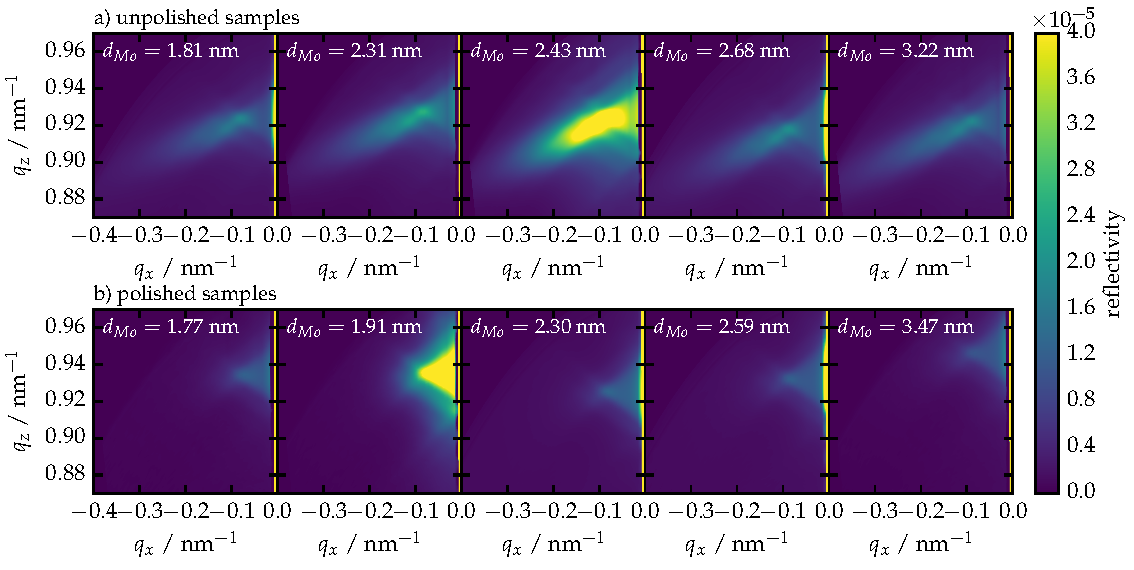
\includegraphics[width=\textwidth]{img/MoSiC_diffuse_measurements}
\caption{Measured diffuse scattering distributions in reciprocal space representation shown on linear false-color scale. The selected unpolished samples are shown in a) with increasing Mo layer thickness $d_{Mo}$. The selected samples for the polished set are shown in b) also in order of increasing Mo thickness $d_{Mo}$. The samples with strongest scattering are shown in larger detail in Fig.~\ref{fig:dwba_data_best_model_comparison}. The diffuse scattering was measured by keeping the detector angle with respect to the incoming beam fixed at $\Delta\Theta = 30^\circ$, while the sample was tilted from an AOI of $\alpha_i=15^\circ$ to $\alpha_i=38^\circ$ with a step size $\Delta\alpha_i = 0.5^\circ$. At each angular position, a wavelength scan from $\lambda=12.35$ nm to $\lambda=14.0$ nm in steps of $\Delta\lambda = 0.01$ nm was performed to map the diffuse scattering distribution.}
\label{ch_diff:fig_mo_si_c_diffuse}
\end{figure*}
The maps in Fig.~\ref{ch_diff:fig_mo_si_c_diffuse}a show the scattering distribution from the unpolished samples marked with the fitted Mo layer thickness as listed in table~\ref{ch_diff:tbl_mo_si_thickness_mcmc_result_selected_samples}. The polished samples are shown in Fig.~\ref{ch_diff:fig_mo_si_c_diffuse}b.

A very prominent observation in both sets, is that one sample in each series shows significantly stronger overall scattering than the others. In addition, both sets show distinctly different scattering distributions clearly differentiating the polished from the unpolished samples. In the case of the polished samples, significantly less scattering can be observed for higher spatial frequencies, whereas more intensity is measured for smaller frequencies. A recognizable characteristic of the off-specular scattering intensity is the observation of a downward tilted Bragg sheet in case of the unpolished samples, which is in contrast to the rocking scan map of the Mo/B$_4$C/Si/C sample from the beginning of this chapter. This is due to a non-orthogonal roughness correlation throughout the stack with respect to the surface and interfaces first observed by \textcite{gullikson_asymmetric_1999}. We have discussed the theoretical aspects of this effect in Sec.~\ref{ch_theo:sec_diffuse_scattering}, but shall investigate this behavior for the specific set of samples studied here.

The downward tilt of the Bragg sheet is clearly observed for all samples in the unpolished series with a similar direction. All samples were measured along the same nominal $x$ axis, i.e.~along the same direction with respect to their mounting orientation during the deposition process. Due to to in-plane measurement of the diffuse scattering, the non-orthogonal roughness correlation angle $\beta$ can only be evaluated along the projection of its directional vector onto the $x$-$z$-plane. However, the vertical correlation direction vector may not necessarily lie in that plane. To verify this property, we shall investigate the corresponding diffuse scattering distribution from the strongest scattering sample with $d_\text{Mo} = \nm{2.43}$ by rotating it by $\SI{90}{\degree}$ around its surface normal onto the sample holder and repeat the mapping of reciprocal space. Fig.~\ref{ch_diff:fig_diffuse_tilt_vs_notilt} shows the comparison of the map obtained earlier with the map from the rotated sample.
\begin{figure*}[htbp]
\centering
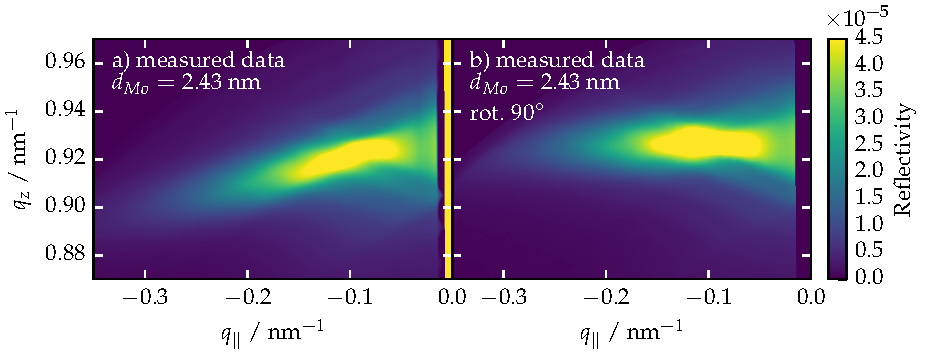
\includegraphics[width=\textwidth]{img/MoSiC_diffuse_tilt_vs_notilt}
\caption{Direct comparison of the measured reciprocal space maps with the DWBA calculation resulting from the parameters obtained with the MCMC optimization procedure (see text). a) shows the maps of the unpolished sample with strongest diffuse scattering. Similarly, b) shows the maps of the polished sample at the respective presumed crystallization threshold with strongest scattering.}
\label{ch_diff:fig_diffuse_tilt_vs_notilt}
\end{figure*}
The tilt direction is clearly different from the map of the rotated sample, we obtain a similarly horizontal Bragg sheet as for the Mo/B$_4$C/Si/C sample in Sec.~\ref{ch_diff:sec_PTB17}. Based on the evaluation of the tilt angle in both maps, it is possible to deduce the direction and total angle $\beta$ of the roughness correlation direction with respect to the surface normal and the orientation directions of the sample during the measurement. This angle is given by the two orthogonally measured Bragg sheet tilt angles $\beta^{\SI{0}{\degree}}$ and $\beta^{\SI{90}{\degree}}$ through
\begin{align}
 \tan^2(\beta) &= \tan^2(\beta^{\SI{0}{\degree}}) + \tan^2(\beta^{\SI{90}{\degree}}) \text{.}
\end{align}
These two independent measurements can be additionally used to verify the results of the reconstruction. We shall thus perform the analysis described in Sec.~\ref{ch_diff:sec_PTB17} and deduce the \gls{psd} parameters including the vertical correlation length as well as the non-orthogonal correlation direction for this sample in particular. For all other measured samples we shall also perform this analysis, where there only the in-planar Bragg sheet tilt angle is determined.

\subsection{Reconstruction of the Interface Morphology}
The theoretical analysis was performed based on the DWBA for all scattering maps measured above. The ideal model for each sample system entering the DWBA calculation was obtained from the analysis in Sec.~\ref{sec:mo_si_model_reconstruction_results}. The optimization functional was calculated according to Eq.~\eqref{eqn:reduced_chi_2} for all off-specular wavelength scans for each angle. The combined likelihood was then calculated similarly to Eq.~\eqref{eqn:total_chi_2_diffuse}, as the sum of all measurement points for all angular positions and wavelengths. The optimization was conducted by the MCMC analysis with respect to the vertical correlation length $\xi_\perp$ in the vertical correlation function $c(q_\parallel)$ and all PSD parameters in $C(q_\parallel)$. The list of the corresponding parameters and their bounds is given in Table~\ref{tbl:diffuse_parameters}.
\begin{table*}
\centering
\caption{Parameters of the DWBA analysis with parameter limits}
\label{tbl:diffuse_parameters}
\begin{tabularx}{\textwidth}{@{}lXll@{}}
\toprule
Parameter & Definition & Lower bound & Upper bound\\ \midrule
$\sigma_r$ / nm & root mean square roughness & $0.0$& $1.0$\\ 
$\xi_\parallel$ / nm & lateral correlation length & $0.0$& $20.0$\\ 
$\xi_\perp$ / nm$^{-1}$ &vertical correlation parameter yielding vertical correlation length trough $\xi_\perp(q_\parallel) = \xi_\perp/q_\parallel^2$ &$0.0$ & $20.0$\\
$\beta$ / $^\circ$&angle for off-axis vertical roughness correlation& $-10.0$ & $10.0$\\ 
 \bottomrule
\end{tabularx}
\end{table*}

For this analysis we assumed a Gaussian roughness profile at the interfaces, which is described mathematically by setting $H\equiv1.0$ for all samples. For the two samples, the full maps with the strongest scattering from each set are shown in comparison to the best model DWBA calculation (Fig~\ref{fig:dwba_data_best_model_comparison}). The results for the roughness of the MCMC analysis are shown in Fig.~\ref{fig:PSD_results}. All values are compiled in Table~\ref{tbl:diffuse_parameters_results}. 
\begin{figure*}[htbp]
\centering
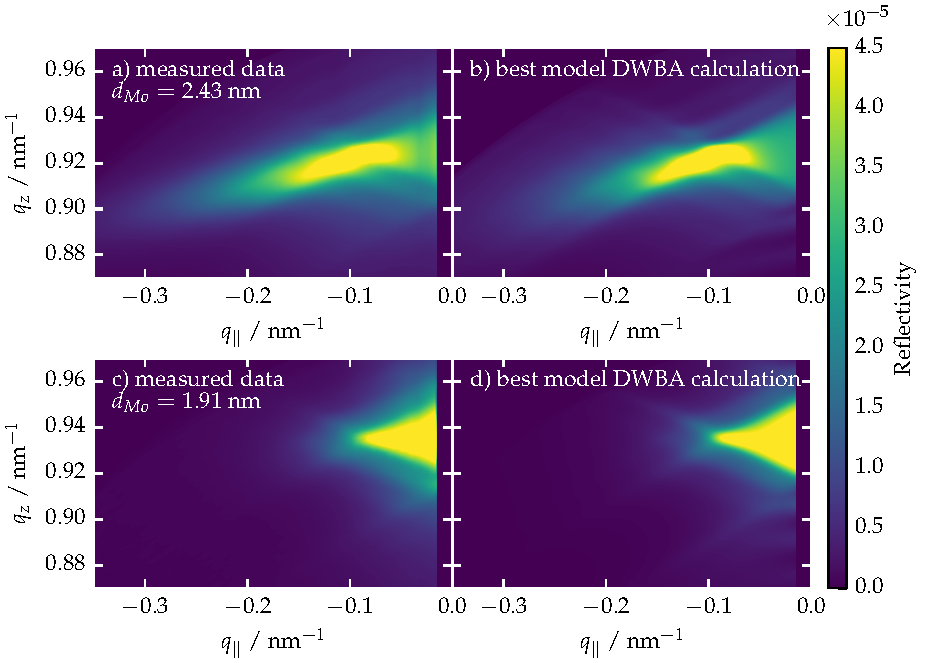
\includegraphics[width=\textwidth]{img/MoSiC_dwba_data_best_model_comparison}
\caption{Direct comparison of the measured reciprocal space maps with the DWBA calculation resulting from the parameters obtained with the MCMC optimization procedure (see text). a) shows the maps of the unpolished sample with strongest diffuse scattering. Similarly, b) shows the maps of the polished sample at the respective presumed crystallization threshold with strongest scattering.}
\label{fig:dwba_data_best_model_comparison}
\end{figure*}

For both sample sets a significant increase of roughness can be observed at the crystallization threshold, which coincides with the lowest reflectance for that sample in each set. Interestingly, the roughness returns to the previous value for further increasing Mo layer thicknesses. The roughening due to the formation of nanocrystallites at the threshold is compensated for even larger thicknesses.
That indicates a smoothing effect due to additional Mo deposition above the crystallization threshold. We also observe a restored peak reflectance in that case. For the polished samples, the formation of crystallites can be observed with similar effects, but at lower Mo layer thickness with overall significantly lower root mean square roughness values.

\begin{table*}[htbp]
\centering
\caption{Results for the DWBA model parameters}
\label{tbl:diffuse_parameters_results}
\begin{tabular}{@{}lllll@{}}
\toprule
nom. Mo thickness / nm&$\sigma_r$ / nm & $\xi_\parallel$ / nm & $\xi_\perp$  / nm$^{-1}$ & $\beta$ / $^\circ$ \\ 
(fitted Mo thickness / nm) & & & &\\ \midrule
\multicolumn{5}{c}{Unpolished samples}\\
\midrule
$1.70$ ($1.81 \pm 0.18$) & $0.227 \pm 0.007$ & $3.14 \pm 0.11$ & $3.69 \pm 0.31$ & $-4.62 \pm 0.11$ \\
$2.21$ ($2.31 \pm 0.22$)& $0.232 \pm 0.005$ & $3.72 \pm 0.09$ & $4.88 \pm 0.35$ & $-5.02 \pm 0.09$ \\
$2.38$ ($2.43 \pm 0.12$) & $0.329 \pm 0.006$ & $4.51 \pm 0.10$ & $4.44 \pm 0.34$ & $-5.67 \pm 0.10$ \\
verification rot.~$90^\circ$ & $0.317 \pm 0.009$ & $4.56 \pm 0.18$ & $3.62 \pm 0.37$ & $+0.55 \pm 0.14$ \\
$2.54$ ($2.68 \pm 0.14$)& $0.211 \pm 0.006$ & $3.61 \pm 0.12$ & $3.80 \pm 0.31$ & $-5.06 \pm 0.12$ \\
$3.05$ ($3.22 \pm 0.12$)& $0.243 \pm 0.005$ & $2.89 \pm 0.06$ & $5.72 \pm 0.31$ & $-5.06 \pm 0.06$ \\
\midrule
\multicolumn{5}{c}{Polished samples}\\
\midrule
$1.70$ ($1.77 \pm 0.20$) & $0.129 \pm 0.006$ & $7.05 \pm 0.38$ & $0.53 \pm 0.05$ & $-1.19 \pm 0.56$ \\
$1.85$ ($1.91 \pm 0.14$)& $0.195 \pm 0.005$ & $10.66 \pm 0.34$ & $0.76 \pm 0.07$ & $-1.50 \pm 0.51$ \\
$2.00$ ($2.30 \pm 0.20$)& $0.105 \pm 0.002$ & $8.95 \pm 0.25$ & $0.76 \pm 0.06$ & $-2.28 \pm 0.30$ \\
$2.30$ ($2.59 \pm 0.13$)& $0.106 \pm 0.003$ & $8.22 \pm 0.29$ & $0.86 \pm 0.08$ & $-2.90 \pm 0.23$ \\
$3.05$ ($3.47 \pm 0.16$)& $0.088 \pm 0.002$ & $10.29 \pm 0.37$ & $1.47 \pm 0.23$ & $-1.62 \pm 0.32$ \\
 \bottomrule
\end{tabular}
\end{table*}

In addition, a large gap between the vertical correlation factors can be observed for comparing the polished and unpolished samples. As is to be expected, the polishing process largely reduces the roughness correlation between different interfaces. In the case of unpolished growth, almost the entire stack is correlated for the observable spatial frequencies. The large values for the in-planar correlation length for the polished samples are also a direct result of the polishing process. 

\subsection{Discussion of the Results}
\begin{figure}[htbp]
\centering
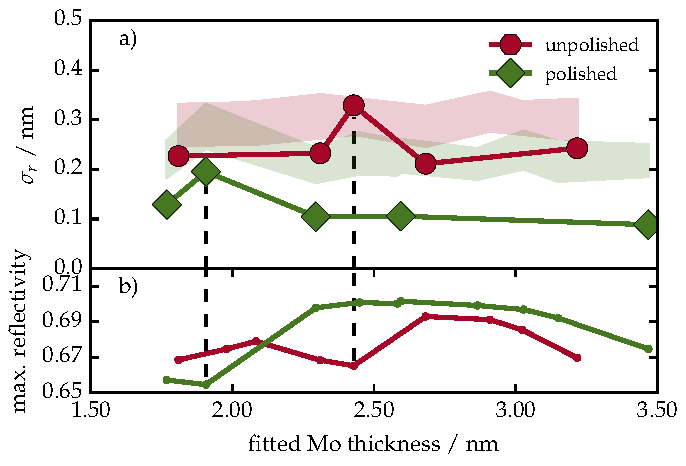
\includegraphics[width=0.7\textwidth]{img/MoSiC_PSD_results}
\caption{a) Root mean square roughness results from the analysis of the diffuse scattering for the two sample sets. In each set, an increase of roughness is observed at the crystallization threshold. For comparison, the max peak reflectance (cf.~Fig.~\ref{fig:EUV_reflectivity}c) for each sample set is shown in b). The increase in roughness clearly correlates with a significant dip in the peak reflectance as indicated by the dashed vertical lines.}
\label{fig:PSD_results}
\end{figure}
We have demonstrated the analysis of Mo/Si/C multilayer systems designed for normal incidence operation in the EUV spectral range. Two sample sets were prepared with a varying Mo layer thickness, while keeping the total period thickness approximately constant. For the second set an interface polishing treatment was applied during deposition of each period to decrease the interface roughness. We have analyzed the thickness of the individual layers in specular EUV and X-ray reflectivity measurements. We observed the designed increase in the Mo content in good agreement with the nominal values. We also observed for both sample sets a simultaneous jump in the total period thickness $D$ and the Mo layer thickness around $d_\text{Mo} = 2.5$ nm for the unpolished samples and $d_\text{Mo} = 2.2$ nm for the polished samples. In comparison to the suspected trend of the peak reflectance with $d_\text{Mo}$ we observed two samples with lower reflectance in both sets, one exactly at the position of this jump and the other sample with nominally $0.15$ nm lower $d_\text{Mo}$. Furthermore, the evaluation of the diffuse scatter revealed increased roughness throughout the ML stack for the samples just at the thickness jump. At least for the unpolished samples, this higher roughness is not observed from evaluating the specular reflectance alone, where the reflectance is diminished by the combined effects of roughness, interdiffusion and compound formation, which is represented by an effective $\sigma$-value in the N\'{e}vot-Croce factor. For the polished samples, the overall effect is smaller and the enhanced scatter is also observed in the total N\'{e}vot-Croce damping factor. The roughness amplitudes as derived from the diffuse scatter, however, have much smaller confidence intervals.

We interpret our findings in line with the observation of the formation of crystallites in the Mo layer \cite{bajt_investigation_2001} at around $2$ nm thickness. Particularly, we assign the threshold to the lower thickness where the reflectance first drops without an observation of increased roughness by diffuse scatter. This is explained (analog to \cite{bajt_investigation_2001}) by the crystallization  process starting with increased interdiffusion and small seeds corresponding to a short correlation length, yielding high spacial frequency roughness, not correlated throughout the stack. The corresponding scatter is thus not resonantly enhanced. Without the enhancement, it is below the detection threshold of our experiment. With increasing crystallites, the diffuse scatter becomes observable at slightly higher Mo thickness. Note that for the unpolished sample, the threshold coincides with the point where the ideal Mo-to-Si ratio should yield the highest reflectance in agreement with the findings in \cite{bajt_investigation_2001}. For the polished samples, this threshold is shifted to thinner Mo layers around $d_\text{Mo} = 1.77(-0.22/+0.19)$ nm. This is beneficial for the peak reflectance, which is higher at the optimum ratio, than for the unpolished set. In both cases, a smoothening occurs for even larger Mo thickness, restoring the roughness to its value below the threshold. The evaluation of the diffuse scatter shows an overall lower roughness for the polished samples and, particularly, a destruction of vertical roughness correlation throughout the stack and an increase of the in-planar correlation length, as intended by the polishing. 

Finally, we note that the analysis methods applied here allow to consistently determine the Mo layer thickness and the average power spectral density roughness for the interfaces throughout the full multilayer stack. The application of these methods to Mo/Si multilayer samples with varying Mo thickness with/without polishing illustrated the power of the method for the investigation of structural changes and confirmed previous findings on the onset of Mo crystallization.

\section{Roughness and Intermixing in Cr/Sc Multilayers} \label{ch_diff:sec_CrSc}
Even in the case of the data, methods and model presented here, the combined 
analysis leaves a correlation between the intermixing parameter $\eta$ and the 
roughness $\sigma_r$, which could not be resolved (see 
Fig.~\ref{fig:eta_sigma_correlation}).
\begin{figure}[htbp]
  \centering
  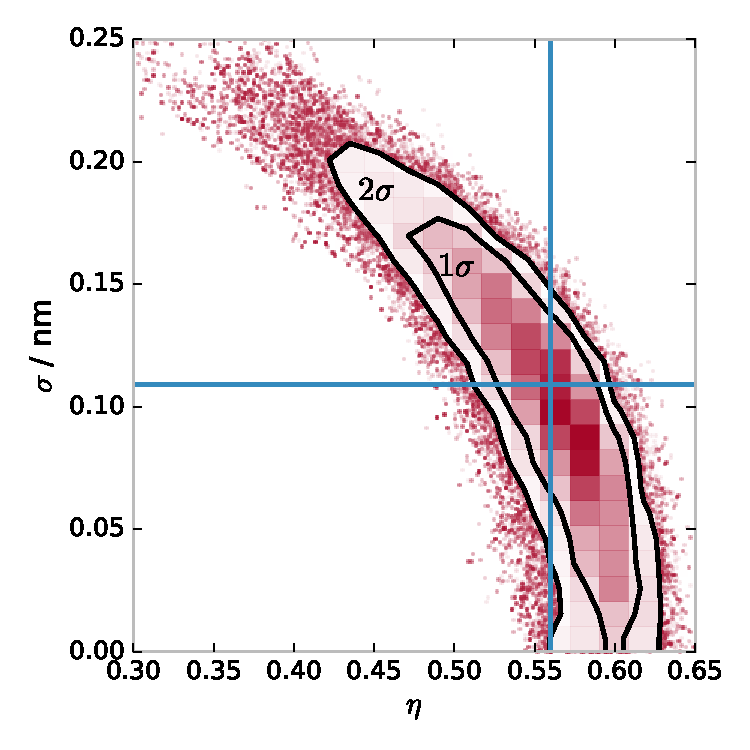
\includegraphics[width=0.5\textwidth]{images/eta_sigma_correlation}
  \caption{Correlation of the projected $\chi^2$ surface onto the parameter 
pair $(\eta, \sigma_r$) by visualization of the position of the MCMC samples in 
the reduced parameter space. The strong correlation of both parameters in the 
optimal solution, which is indicated by blue solid lines, is clearly visible. 
The percentiles corresponding to one and two standard deviations $\sigma$ are 
indicated by the black contour lines.}
  \label{fig:eta_sigma_correlation}
\end{figure}
This means that none of the methods, not even the combined analysis, contains 
sufficient information to deduct an unambiguous result for the roughness or 
intermixing. Intermixing alone merely reduces optical contrast, whereas 
interface roughness causes diffuse scattering. One should be able to 
distinguish between the two through the measurement of the diffuse scattering. 
The distribution of the off-specular scattering with respect to the scattering 
angle and wavelength provides additional information on the vertical and 
lateral correlation of spatial roughness frequencies. The latter is described 
by the power spectral density. We conducted a diffuse scattering experiment as 
described in Sec.~\ref{sec:experimental}. The analysis was conducted based on 
the DWBA formalism outlined in Sec.~\ref{sec:matrix_formalism}. The subfigures 
(a) and (b) of Fig.~\ref{fig:diffuse_meas} show the measured reciprocal space 
map in direct comparison to the best model found within the DWBA approach.
\onecolumn
\begin{figure}[htbp]
  \centering
  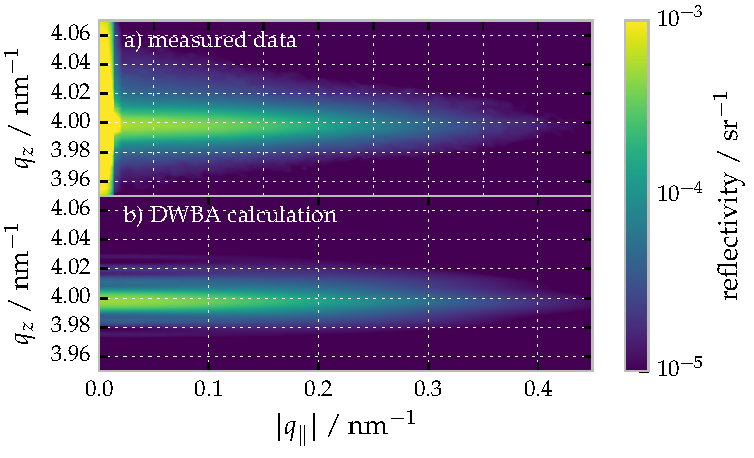
\includegraphics[width=0.7\textwidth]{img/CrSc_diffuse_measured_vs_dwba}
  \caption{a) Diffuse scattering measurement in $q$-space representation and 
log scale. b) DWBA calculation of the optimal PSD model based on the electron 
density profile with the multilayer parameters for the combined analysis listed 
in Table~\ref{tbl:results}.}
  \label{fig:diffuse_meas}
\end{figure}

\begin{figure}[htbp]
  \centering
  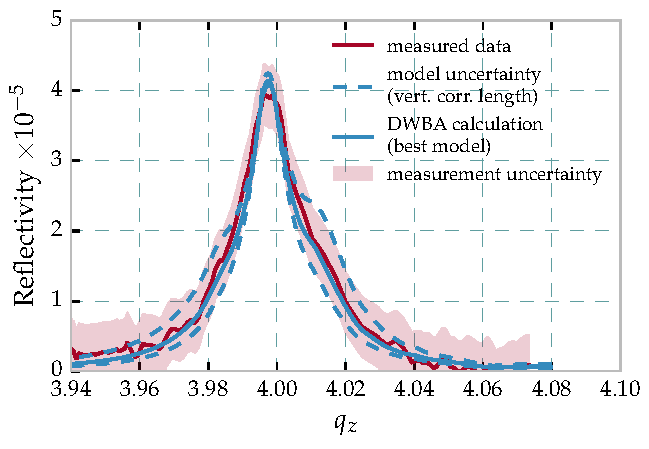
\includegraphics[width=0.7\textwidth]{img/CrSc_diffuse_vertical_correlation}
  \caption{ Vertical cut at the indicated white dashed cut 
positions in (a) and (b). The blue dashed lines show two limiting cases for the 
value of the vertical correlation length. The result is a model uncertainty in 
the PSD.}
  \label{fig:diffuse_meas}
\end{figure}

\begin{figure}[htbp]
  \centering
  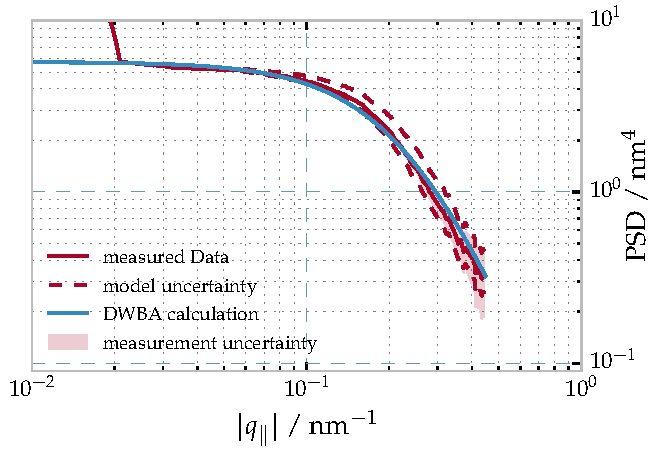
\includegraphics[width=0.7\textwidth]{img/CrSc_diffuse_PSD}
  \caption{Comparison of the extracted effective PSDs from the diffuse 
scattering measurement (Measured Data) shown in (a) and the DWBA calculation of 
(b) at the horizontal cut positions indicated by the white dashed lines. The 
uncertainty interval for the extracted power spectral density is shown by the 
two dashed PSD profiles (see main text).}
  \label{fig:diffuse_meas}
\end{figure}


The formation of a narrow Bragg sheet \cite{haase_role_2014,salditt_kinetic_1994} 
confirms the high degree of roughness correlation and thereby justifies the 
approximations made in Sec.~\ref{sec:matrix_formalism} for identical roughness 
properties at each interface. To deduct the effective power spectral density 
shown in Fig.~\ref{fig:diffuse_meas}(c), we have taken a cut along the Bragg 
sheet as indicated by the horizontal white dashed lines in the reciprocal space 
maps. We divided the extracted scattering intensity by the multilayer 
enhancement factor in Eq.~\ref{eqn:dwba}, leaving the contribution of the 
effective PSD $C(q_\parallel)$ to the diffuse scattering.
This requires that the vertical correlation factor $\xi_\perp$ be determined 
first, which enters the calculation of the multilayer enhancement factor 
through the replication factor in Eq.~\eqref{eqn:vertical_correlation}. Due to 
the very high computational cost of a MCMC procedure, we have instead 
calculated two limiting cases of the vertical correlation. This was done by 
analyzing the width of the Bragg sheet at the vertical white dashed cut 
positions, indicated in Fig.~\ref{fig:diffuse_meas}(a,b), and comparing the 
simulated intensity distribution with the measurement uncertainty. The two 
limiting cases are shown in Fig.~\ref{fig:diffuse_meas}(d) (blue dashed curves) 
including the best model (solid blue curve) in comparison with the measured 
data (solid red curve). Proceeding from here, we have evaluated the measured 
PSD with the corresponding multilayer enhancement factor as described above. 
Again, the two limiting cases are shown as red dashed curves in 
Fig.~\ref{fig:diffuse_meas}(c) including the PSD deduced from the best model 
value for $\xi_\perp$ as a solid red curve. The root mean square (r.m.s.) 
roughness deducted from these PSDs is given by the two-dimensional integral as
\begin{align}
\sigma_r &=\frac{1}{2\pi} \sqrt{\int_{0}^{\infty} q_\parallel C(q_\parallel) \, 
dq_\parallel} \text{.}
\end{align}
The uncertainty of the PSD due to the vertical correlation leads to an 
uncertainty in the r.m.s. roughness when evaluating the integral. Due to the 
limited $q_\parallel$ range where measurements can be taken, we have fitted the 
PSD model of Eq.~\eqref{eqn:psd} to the three resulting PSDs and performed the 
integration over the full $q_\parallel$ range. The deviation of the integration 
for the PSD model fit and the data in the available range were negligible. The 
best model results for the vertical replication factor and the power spectral 
density are given in Table.~\ref{tbl:psd_results}, together with their 
uncertainties resulting from the described procedure. The best fit of the PSD 
model is shown in Fig.~\ref{fig:diffuse_meas}(c) as a solid blue curve.
\begin{table}
\centering
\caption{Best model parameters of the PSD as a result of the diffuse scattering 
analysis}
\label{tbl:psd_results}
\begin{tabular}{@{}ll@{}}
\toprule
Parameter & Best model values\\ \midrule
$\sigma_r$ / nm & $0.17 \pm 0.02$ \\
$\xi_\parallel$ / nm& $4.00 \pm 0.35$ \\
$\xi_\perp$  / nm$^{-1}$& $10.5 \pm 3.5$ \\
$H$ & $1.0$ \\
$\beta$ & $0.0$ \\
 \bottomrule
\end{tabular}
\end{table}
The r.m.s.~roughness value found with the analysis of the diffuse scattering is 
identical within its uncertainty interval to the value obtained from the 
combined analysis and thus confirms the intermixing and roughness parameters 
listed in Table.~\ref{tbl:results}.
